\chapter{Background}
\label{ch:background}

    \section{Computing Continuum}
    \label{sec:computing-continuum-background}

        Placeholder

    \section{Scheduling and Adaptation}
    \label{sec:scheduling-and-adaptation-background}

    \section{Prediction of Load}
    \label{sec:prediction-of-load-background}

    \section{Recurrent Neural Network}
    \label{sec:rnn-background}

        Recurrent neural networks (RNN) were designed to improve upon the shortcomings of traditional neural networks when dealing with sequential data.
        
        
        \subsection{Recurrent Cell Architecture}
        \label{sec:recurrent-cell-architecture-background}

            A traditional feed-forward neural network (FNN) is unidirectional, meaning that they have a single direction and hence cannot persist information over a time step $t$.
            Looping structures are added to a feed-forward neural network that enable the persistance of information about time-series or sequential data. 
            This is the reason RNN's are known as "recurrent" neural networks.
            \begin{figure}[h!]
                \centering
                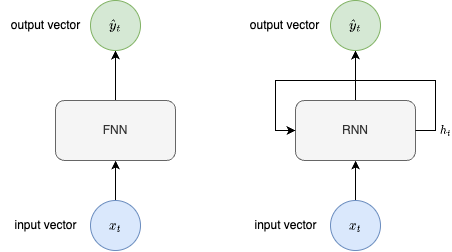
\includegraphics[scale=0.5]{figures/FNN_vs_RNN.drawio.png}
                \caption{FNN vs. RNN}
                \label{fig:fnn-vs-rnn}
            \end{figure}
            As can be seen in figure \ref{fig:fnn-vs-rnn}, the RNN has an additional loop inside it to persist time-series information. The loop structure enables the RNN to apply a \emph{recurrence relation} (see \ref{sec:recurrence-relation-background}) at every time step in order to process a sequence.

            The rectangle containing the "RNN" label is defined as a "recurrent cell".
            This workflow of a single RNN cell can be seen in more detail in figure \ref{fig:single-rnn-cell}, where the previous cell state $h_{t-1}$ and the current input $x_t$ are used as the input of the recurrent cell, get combined and forwarded to the $tanh$ \emph{activation function}, which returns the output vector $\hat{y}_t$ and $h_t$ (the recurrence relation).

        \subsection{Recurrence Relation}
        \label{sec:recurrence-relation-background}

            The recurrence relation is applied at every time step to process a sequence.

            The recurrent relation seen in figure \ref{fig:fnn-vs-rnn} is denoted as $h_t$, and is defined as $h_t = f_w(h_{t - 1}, x_t)$, where $f_w$ is a function that is parametrized by the weights, $h_{t-1}$ is the previous state and $x_t$ is the input vector at time step $t$. With the addition of $h_{t-1}$, the model is now also taking the previous time step into account when updating the current time step. 
            The recurrence relation in a more mathematical notation is:

            $$h_t = \tanh(W^T_{hh} h_{t-1} + W^T_{xh} x_t)$$

            Both the input vector $x_t$ as well as the previous state $h_{t-1}$ are multiplied with the two separate weight matrices $W^T_{xh}$ and $W^T{hh}$ respectively, combined and fed to the $\tanh$ activation function. Finally, the $\tanh$ function returns the output vector $\hat{y}_t$ at time step $t$.

            \begin{figure}[h!]
                \centering
                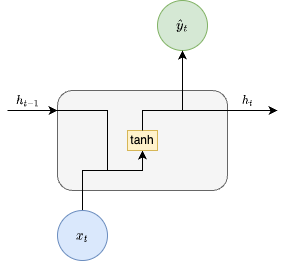
\includegraphics[scale=0.5]{figures/single_rnn_cell.drawio.png}
                \caption{Single RNN Cell}
                \label{fig:single-rnn-cell}
            \end{figure}

        \subsection{RNN Loop Unfolding}
        \label{sec:rnn-loop-unfolding-background}

            Placeholder

        \subsection{Shortcomings of RNNs}
        \label{sec:shortcomings-of-rnns-background}
            
            Placeholder

    \section{Long-Short Term Memory}
    \label{sec:lstm-background}

        \emph{Long-Short Term Memory (LSTM)} are a type of \ref{sec:rnn-background} but improve upon the shortcomings of regular RNN models.
        LSTMs are best suited for learning long term dependencies in sequential or time-series data.

        The introduction of \emph{self-looping} to produce paths is the main architectural improvement for LSTMs over RNNs. This additional component diminishes the problem of the vanishing gradients problem and enables gradients to flow for a long duration.